\documentclass[11pt]{beamer}
\usetheme{CambridgeUS}
\usecolortheme{lily}
\usepackage[utf8]{inputenc}
\usepackage{amsmath}
\usepackage{amsfonts}
\usepackage{amssymb}
\usepackage{outlines}
\usepackage{graphicx}
\usepackage{xcolor}
\newcommand{\indep}{\rotatebox[origin=c]{90}{$\models$}}
\usepackage[numbers]{natbib}
\usepackage{pdflscape}
\usepackage{booktabs}
\usepackage{caption}
\usepackage{dcolumn}
\captionsetup{skip=0.333\baselineskip}
\newcolumntype{d}[1]{D{.}{.}{#1}}
\newcommand\mc[1]{\multicolumn{1}{@{}c@{}}{#1}} % handy shortcut macro
\bibliographystyle{acm}
\author{Julio B. Roll}
\title{Heterogeneous Innovation and Intertemporal Productivity Choice}
%\subtitle{}
\setbeamercovered{transparent} 
\definecolor{brightmaroon}{rgb}{0.76, 0.13, 0.28}
\setbeamercolor{frametitle}{fg=brightmaroon}
\setbeamercolor{title}{fg=brightmaroon}
\setbeamertemplate{navigation symbols}{} 
%\logo{} 
%\institute{} 
\date{February 5, 2018} 
%\subject{} 

\AtBeginSection[]{
  \begin{frame}
  \vfill
  \centering
  \begin{beamercolorbox}[sep=8pt,center,shadow=true,rounded=true]{title}
    \usebeamerfont{title}\insertsectionhead\par%
  \end{beamercolorbox}
  \vfill
  \end{frame}
}

\begin{document}

\begin{frame}
	\maketitle
\end{frame}

\begin{frame}{Research Motivation}
	Since the rebirth of endogenous growth in mid-2000s, literature became richer:
	\begin{itemize}\itemsep12pt
	\item Classics: Romer (1990), Grossman and Helpman (1991), Aghion and Howitt (1992);
	\item Micro-data renewal: Klette and Kortum (2004), Lentz and Mortensen (2008);
	\item Current state of the art: Acemoglu et al. (2013), Akcigit and Kerr (2016).
	\end{itemize}
$\Rightarrow$ We now account for creative destruction/turnover, R\&D spillover, imitation, incumbents' innovation, firm heterogeneity...but...
\end{frame}

%being generous: riskless rate not added, only sales - cogs, other expenses lacking

\begin{frame}{Research Motivation}
	\begin{center}
	\begin{figure}\centering\label{Ratio_firms}
	  \fbox{\resizebox{3.8in}{2.6in}{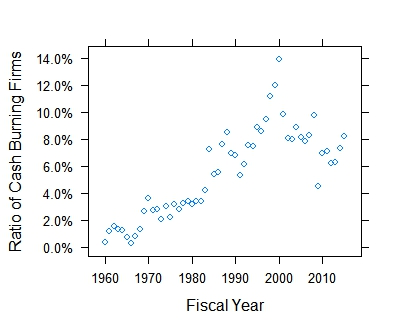
\includegraphics{Ratio_firms.jpeg}}}
	\end{figure}
	\end{center}
\end{frame}

\begin{frame}{Research Motivation}
	\begin{center}
	\begin{figure}\centering\label{Ratio_emp}
	  \fbox{\resizebox{3.8in}{2.6in}{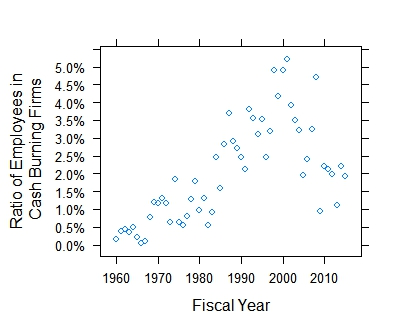
\includegraphics{Ratio_emp.jpeg}}}
	\end{figure}
	\end{center}
\end{frame}

\begin{frame}{Research Motivation}
	\textbf{Questions:}
	\begin{itemize}\itemsep12pt
		\item What's the impact of intertemporal TFP choice on aggregate TFP?
		% (short-term, long-term)
		\item What are the implications to the innovation strategy of firms? 
		\item How long does it take to "get TFP back"?
		%time span of intertemporal change cycle
	\end{itemize}	 
	\textbf{Why is it interesting?}
    \begin{itemize}\itemsep12pt
	\item Having Bluetooth in your car $\neq$ Tesla, or innovation heterogeneity sparks different firm behavior;
	%especially abrupt innovation
	\item Less TFP now for more TFP latter could impact aggregate measurement;
	\item Finance has a role in "footing the bill" and reallocation;
	\item Normative: how to spur abrupt innovation?
	\end{itemize}
\end{frame}

%"say I'm Toyota...", product life-cycle

\begin{frame}{Framework - Innovation}
	\textbf{Focus:} Innovation: internal (incremental or abrupt), external, and entrants (the last two only abrupt).
	%my contribution (internal innovation = higher markups)
	\begin{center}
	\begin{figure}\centering\label{Innov2}
	  \fbox{\resizebox{3.2in}{2.2in}{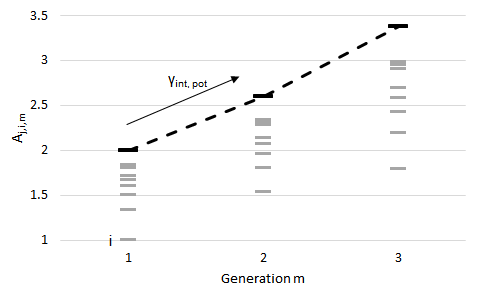
\includegraphics{Innov_2.png}}}
	\end{figure}
	\end{center}
\end{frame}

\begin{frame}{Framework - Innovation}
	\textbf{Focus:} Innovation: internal (incremental or abrupt), external, and entrants (the last two only abrupt).
	%my contribution (internal innovation = higher markups)
	\begin{center}
	\begin{figure}\centering\label{Innov3}
	  \fbox{\resizebox{3.2in}{2.2in}{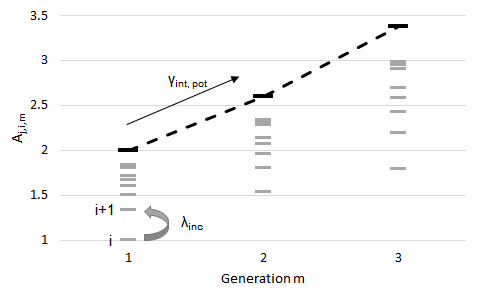
\includegraphics{Innov_3.png}}}
	\end{figure}
	\end{center}
\end{frame}

\begin{frame}{Framework - Innovation}
	\textbf{Focus:} Innovation: internal (incremental or abrupt), external, and entrants (the last two only abrupt).
	%my contribution (internal innovation = higher markups)
	\begin{center}
	\begin{figure}\centering\label{Innov4}
	  \fbox{\resizebox{3.2in}{2.2in}{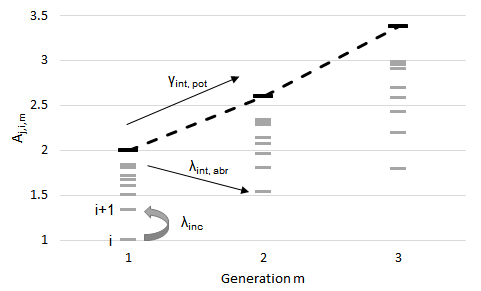
\includegraphics{Innov_4.png}}}
	\end{figure}
	\end{center}
\end{frame}

\begin{frame}{Framework - Innovation}
	\textbf{Focus:} Innovation: internal (incremental or abrupt), external, and entrants (the last two only abrupt).
	%my contribution (internal innovation = higher markups)
	\begin{center}
	\begin{figure}\centering\label{Innov5}
	  \fbox{\resizebox{3.2in}{2.2in}{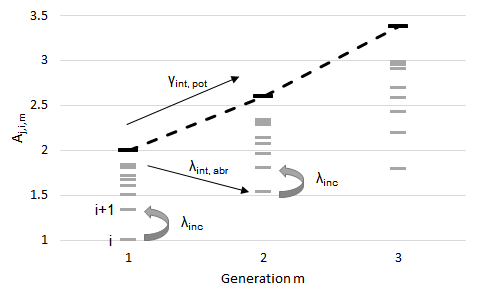
\includegraphics{Innov_5.png}}}
	\end{figure}
	\end{center}
\end{frame}

\begin{frame}{Framework - Innovation}
	\textbf{Focus:} Innovation: internal (incremental or abrupt), external, and entrants (the last two only abrupt).
	%my contribution (internal innovation = higher markups)
	\begin{center}
	\begin{figure}\centering\label{Innov6}
	  \fbox{\resizebox{3.2in}{2.2in}{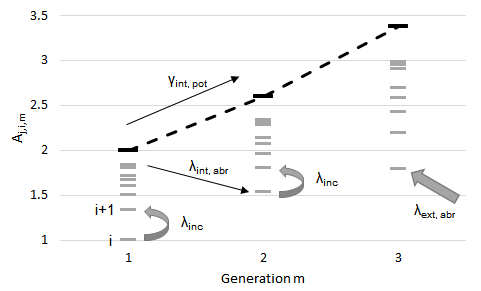
\includegraphics{Innov_6.png}}}
	\end{figure}
	\end{center}
\end{frame}

\begin{frame}{Framework - Innovation}
	\textbf{Focus:} Innovation: internal (incremental or abrupt), external, and entrants (the last two only abrupt).
	%my contribution (internal innovation = higher markups)
	\begin{center}
	\begin{figure}\centering\label{Innov7}
	  \fbox{\resizebox{3.2in}{2.2in}{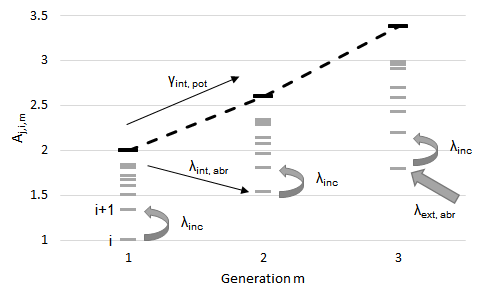
\includegraphics{Innov_7.png}}}
	\end{figure}
	\end{center}
\end{frame}

\begin{frame}{Framework - Innovation}
	\begin{itemize}\itemsep10pt	
	\item Law of motion: $A_{t+\Delta t} =\begin{cases}
               A_m(1+\alpha^{s})\:,\: \lambda_{inc}\Delta t \:,\: \alpha \in (0,1)\:,\:\ s \in \{1, 2, ...\}\\
               A_t\gamma_{int,abr}\:,\: \lambda_{int,abr}\Delta t\\
               A_t \:, \: \big[1 - \lambda_{inc}\Delta t; 1 - \lambda_{int,abr}\Delta t\big] 
    \end{cases}$
	\item Incremental R\&D cost: $\psi_{inc}(\lambda_{inc}, A_{t}) = \xi_j A_t \lambda_{inc}^{\eta}$
	\item Catching-up: laggards pay $\psi_{inc}(\lambda_{inc}, A_{t})$ and get an arrival $\lambda_{inc} + h$;
	\item Abrupt R\&D cost (for $n_p > 0$): $\psi_{abr}(\lambda_{ext,abr}, \bar{A}_{t}) = \xi_j \bar{A}_t \lambda_{ext,abr}^{\eta}\:$, $\bar{A}_{t}$ sector average;
	%average, to eliminate dependence on R&D level (cst fraction of total expenditure), levels out with returns
	\item Cournot competition: profits $\pi_t$ scale with $\frac{A_{j,i,m}}{\sum_{j}A_{j,i,m}}$ within an industry.
	\end{itemize}
\end{frame}

\begin{frame}{Framework - Innovation}
Outside entrepreneur:
	\begin{itemize}\itemsep12pt	
	%present value eq: of max (dividends, returns) discounted with r
	%rP = D + delP/del t: del = capital gains, D dividends
	\item Value function: $rV_0 - \dot{V}_0 = \max\limits_{\lambda_{ext, abr}}\big[\lambda_{ext, abr}\big[E_j\big[V(A_{t, m+1})\big] - V_0\big] - v \bar{A}_{t}\lambda_{ext, abr}\big]$
 	\item Cost: $C_E(\lambda_{ext, abr}, \bar{A}_{t}) = v \bar{A}_{t} \lambda_{ext, abr}\:$, $v$ a constant;
	\item Free entry condition: $E_j\big[V(A_{t, m+1})\big] = v \bar{A}_{t}$
	\item $\Rightarrow$ Each firm faces an aggregate endogenous creative destruction (CD) of rate $\tau_{CE}$ and internal competition rate $\tau_I$.
	\end{itemize}
\end{frame}

\begin{frame}{Framework - Innovation}
Incumbents:
	\begin{itemize}
	\item Value function: $rV(A_t) - \dot{V}(A_t) =$\vspace{-3mm} $$ \max_{\substack{\lambda_{inc},\:\lambda_{int, abr}\\\lambda_{ext, abr}}}\left[\begin{aligned}
		&\sum_k^{n_{j, p}}\left[\begin{aligned}
			&\qquad\quad\pi_t n_{j, p} - \{\xi_j\lambda_{inc}^{\eta}A_{t,m};\xi_j\bar{A}_t\lambda_{int, abr}^{\eta}\}\\
			&\ \ + \{\lambda_{inc}\big[V(A_{t,m}^{k-}\cup A_{t+\Delta t,m}^{k}) - V(A_{t,m})\big];\\
			& \lambda_{int, abr}\big[E_j\big[V(A_{t,m}^{k-}\cup A_{t+\Delta t,m+1}^{k}\big] - V(A_{t,m})\big]\}\\
			&\quad\ \ - \tau_I\big[V(A_{t,m}\setminus \bar{A}_{t+\Delta t,m}^{k}) - V(A_{t,m})\big]\\
			&\quad- \tau_{CE}\big[V(A_{t,m}\setminus\bar{A}_{t+\Delta t,m+1}^{k}) - V(A_{t,m})\big]
		\end{aligned}\right]\\
		&\quad+ \lambda_{ext, abr}\big[E_j\big[V(A_{t,m}^{k}\cup A_{t+\Delta t,m+1}^{k'}\big] - V(A_{t,m})\big]\\
		&\qquad\qquad\qquad\quad- \xi_j\bar{A}_t\lambda_{int, abr}^{\eta} - \Phi\bar{A}_t
	\end{aligned}\right]$$
	\end{itemize}
	\vspace{-3mm}
	\begin{columns}
	\begin{column}{0.5\textwidth}
	\begin{itemize}\itemsep3pt	
   	\item 1\textsuperscript{st}: instant returns - costs;
	\item 2\textsuperscript{nd}, 3\textsuperscript{rd}: return from int. R\&D;
	\item 4\textsuperscript{th}: internal competition;
	\end{itemize}
	\end{column}
	\begin{column}{0.5\textwidth}
	\begin{itemize}\itemsep3pt	
	\item 5\textsuperscript{th}: external CE;
	\item 6\textsuperscript{th}: return from abr. R\&D;
	\item 7\textsuperscript{th}: Abr. R\&D and fixed costs;
	\end{itemize}    
	\end{column}
	\end{columns}			
\end{frame}

\begin{frame}{Empirical Work - Patents}
How to discipline $\{\alpha, \gamma_{int, abr}, \gamma_{ext,abr},\gamma_{int, pot}\}$?
	\begin{itemize}\itemsep12pt	
		\item USPTO patent data (e.g. \# patents, \# patent citations, if it's self-citation or external...).
		%data linked to Compustat
	\end{itemize}
Model (complete):
	\begin{itemize}
		\item Endogenous: R\&D, productivity (all parameters);
		\item Exogenous: labor market (wages, supply), consumers (discounting), mass of entrants;
		\item Estimated (for Patents): $\{\alpha, \gamma_{int, abr}, \gamma_{ext,abr},\gamma_{int, pot}\}$;
		\item Calibrated (for Complete version): discounting, curvature of the R\&D cost function ($\eta$);
	\end{itemize}
\end{frame}

\begin{frame}{Empirical Work - Patents}
Estimation strategy:
	\begin{itemize}\itemsep12pt	
		\item Patent and citation distribution: invariant (at SS);
		\item Need to discipline patent arrival and quality ladder;
		\item Find the "decay rate" of patent quality;
		\item Distinguish external vs. internal (type of citation), abrupt vs. incremental (\# of citations);
		\item Generational productivity step: impose the same shape and compare absolute levels ("envelope").
		%ideally: product cycle data
	\end{itemize}
\end{frame}

\begin{frame}{Conclusion}
\begin{itemize}\itemsep12pt	
		\item Goal: estimate the R\&D part of an endogenous growth model with heterogeneous innovation;
		\item Possibilities: 
		\begin{itemize}\itemsep12pt
			\item Add firm-level financials and estimate the parameters of the Partial Equilibrium (indirect inference);
			\item Solve the SS;
			\item Cure cancer...
		\end{itemize}
		\item Caveats: lots of firms don't innovate, patents do not represent innovation (nor products, ideally we would have product-level data).
	\end{itemize}
\end{frame}

\begin{frame}{References}
	\nocite{*}
	\bibliography{SE-Proposal}
\end{frame}

\end{document}